\chapter{Diseño e implementación}

\label{Chapter3}

En el presente capítulo se presentan los detalles del diseño y los criterios adoptados para el desarrollo del trabajo junto con los pasos seguidos para su implementación.

\section{Arquitectura del sistema}

El sistema tiene una configuración de arquitectura del tipo cliente-servidor. Está constituido por dos nodos y un servidor, los cuales están conectados a la red local y se comunican a través del protocolo MQTT. El servidor recibe los parámetros actuales de estado y cambios desde cada dispositivo, los procesa y almacena en la base de datos. También envía mensajes hacia los dispositivos para cambiar el estado de las salidas o el parámetro que se desee cambiar. Los usuarios pueden consultar y modificar el estado de los dispositivos desde un navegador web móvil o desde una computadora.

En la figura \ref{fig:9} se puede observar la arquitectura cliente-servidor del sistema implementado en el trabajo.

\begin{figure}[h]
\centering
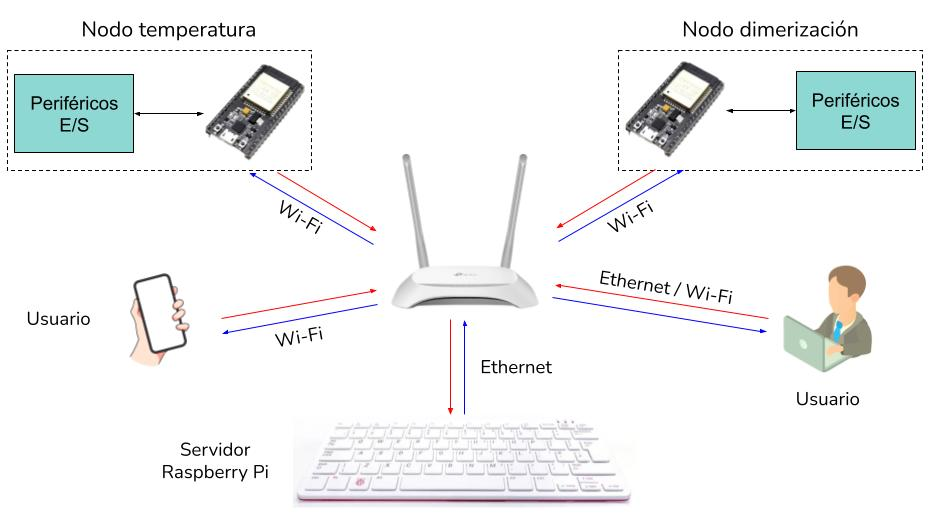
\includegraphics[scale=0.4]{Imagen 9 - cliente-servidor.jpg}
\caption[Arquitectura cliente-servidor]{Arquitectura cliente-servidor. \footnotemark}
\label{fig:9}
\end{figure}
\footnotetext{Imagen tomada de: \url{https://www.bujarra.com/raspberry-pi-servidor-vpn-con-pptp/}}

Uno de los nodos tiene como función sensar y controlar de temperatura de un recinto, y el otro controlar la iluminación. Originalmente el proyecto estaba pensado para que un solo nodo implemente estas dos funciones, pero durante el desarrollo se optó por la implementación separada. Este cambio se basó en la idea de modularizar los nodos y que sus funciones sean específicas. De esta forma es más amigable para el usuario visualizar y modificar el estado en pantalla e implementar el alta de nuevos dispositivos en el sistema.

El servidor está montado sobre una Raspberry Pi 400 con un sistema operativo Raspbian con interfaz gráfica. Este sistema operativo es la versión oficial ofrecida por la fundación Rasperry Pi y está basado en Debian versión 11 (\textit{bullseye}). En esta etapa de desarrollo se optó por una Raspberry Pi 400 por una cuestión de costos y practicidad a la hora de desarrollar y hacer las pruebas, aunque tiene un mayor volumen que los otros modelos de la familia. Al momento de ofrecer una solución definitiva está pensado que sea implementado en una placa con el formato más pequeño como cualquiera de las Raspberry Pi 4. La conexión del servidor a la red local es por cable Ethernet.

\subsection{Especificaciones técnicas del servidor}

El sistema operativo del servidor está instalado y se ejecuta desde un disco de estado sólido por USB. Este tipo de discos tienen una mayor capacidad de escrituras y lecturas que una memoria microSD, lo que resulta favorable al momento de hacer modificaciones y pruebas de ejecución de software. En la versión final del sistema todo el software estará instalado en una tarjeta microSD para que todo el conjunto sea lo más pequeño posible.

En la tabla \ref{tab:Especificaciones Raspberry Pi 400} pueden verse las especificaciones técnicas de hardware más importantes del modelo Raspberry Pi 400.

\begin{table}[h]
\centering
\caption[Raspberry Pi 400]{Especificaciones de Raspberry Pi 400.}
\begin{tabular}{l c}
\toprule
Procesador		&	Broadcom BCM2711 quad-core Cortex-A72(ARM v8) \\
				&	64-bit SoC @ 1.8GHz \\
\midrule
Memoria			&	4GB LPDDR4-3200 \\
\midrule
				&	2.4GHz and 5.0GHz 802.11b/g/n/ac wireless LAN \\
Conectividad		&	Bluetooth 5.0, BLE\\
				&   Gigabit Ethernet \\
\midrule
Alimentación		&	5V DC vía USB-C\\
\bottomrule
\hline
\end{tabular}
\label{tab:Especificaciones Raspberry Pi 400}
\end{table}

\section{Modelo de datos}

En esta sección se describen las diferentes tablas dentro de la base de datos de tipo relacional MariaDB. Con el objetivo de mostrar una representación visual fácil de comprender se muestran las imágenes representadas en la página phpMyadmin. Las tablas que forman dicha base son:

\begin{itemize}
	\item Dispositivos.
	\item Usuarios.
	\item Mediciones.
\end{itemize}

Debe tenerse en cuenta que todo el contenido que se ejecuta del lado del servidor se encuentra dentro de un contenedor Docker. Dicho contenido corresponde a las imágenes de los servicios de Ionic, MariaDB, phpMyAdmin, backend con Node y mosquitto. En la figura \ref{fig:10} se observa el contenido del archivo \textit{docker-compose.yml} pertinente a la configuración de los servicios de MariaDB y phpMyAdmin.

\begin{figure}[h]
\centering
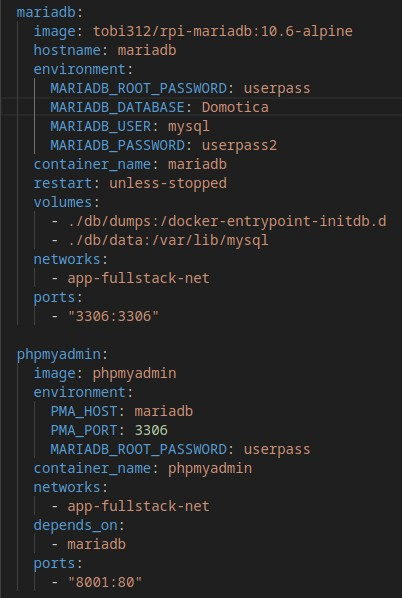
\includegraphics[scale=0.6]{Imagen 10 - Docker base datos.jpg}
\caption[Docker base datos]{Configuración de Docker de la base de datos. \footnotemark}
\label{fig:10}
\end{figure}

\subsection{Tabla Dispositivos}

Esta tabla contiene los datos de los dispositivos dados de alta en el sistema. Dichos datos son el ID del dispositivo, el nombre, la ubicación, la dirección MAC, el tipo, el valor de la alarma y el estado de la alarma (0 para desactivada y 1 para activada).

En la figura \ref{fig:11} puede verse la tabla cargada con 2 dispositivos funcionando.

\begin{figure}[h]
\centering
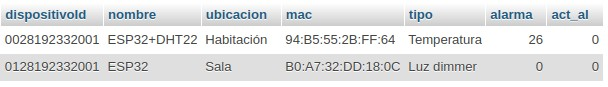
\includegraphics[scale=0.6]{Imagen 11 - Tabla dispositivos.jpg}
\caption[Tabla dispositivos]{Tabla de dispositivos. \footnotemark}
\label{fig:11}
\end{figure}

El ID del dispositivo es un número brindado por el fabricante del dispositivo que consta de 13 números y está formado por: los primeros 2 dígitos que corresponden al tipo de dispositivo (el sistema está pensado para cubrir hasta un total de 100 tipos de dispositivos, aunque en esta etapa de prototipo sólo se hayan desarrollado 2); 4 dígitos de seguridad fijos que en este caso son "2819" y sirven para corroboración y como seguridad; y los últimos 5 dígitos corresponden al número de serie del equipo (2 para el año, 2 para la semana y 3 para el número de fabricación del equipo en esa semana, en ese orden). Como puede observarse, el sistema está pensado para que en un futuro sea parte de una producción en serie.

Tanto el nombre como la ubicación son campos alfanuméricos elegidos por el usuario para describir al dispositivo. La dirección MAC es enviada por el dispositivo la primera vez que se conecta al sistema y no se completa por el usuario. El tipo corresponde al tipo de sensor y para esta etapa del desarrollo puede ser "Temperatura" o "Luz dimmer".

El valor de la alarma es un campo numérico y sólo tiene efecto para dispositivos del tipo de temperatura. Se enviará una notificación por mail cada vez que el valor enviado por el dispositivo sea mayor o igual al seteado en este campo, siempre que dicha alarma esté activada en el campo.

\subsection{Tabla Usuarios}

La tabla de usuarios contiene todos los datos relacionados a aquellas personas que vayan a utilizar el sistema. En esta etapa está implementado con 3 usuarios, ya que al ser de tipo hogareño resultaría difícil que más de 3 personar dentro de una misma casa se registren. Pero con pocos cambios el sistema podría ser escalable a la cantidad de usuarios que se desee, generando una página de alta de usuarios.

Los valores almacenados en esta tabla son el ID de usuario (de 1 a 3), el nombre de usuario, la clave, el nombre de la persona y su apellido, su e-mail y un campo de tipo booleano que se modificará cuando se haya actualizado por primera vez. Cabe aclarar que cada vez que se ingrese al sistema con un usuario que no haya actualizado sus datos, se mostrará en pantalla un aviso para que este actualice sus datos.

En la figura \ref{fig:12} puede verse la tabla cargada con los 3 usuarios de los cuales hay 2 actualizados y el tercero tiene los valores por defecto.

\begin{figure}[h]
\centering
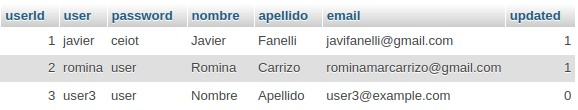
\includegraphics[scale=0.6]{Imagen 12 - Tabla usuarios.jpg}
\caption[Tabla usuarios]{Tabla de usuarios. \footnotemark}
\label{fig:12}
\end{figure}

\subsection{Tabla Mediciones}

La tabla de mediciones contiene todos los datos referentes a las mediciones realizadas por los dispositivos y los datos de modo seleccionado. Los dispositivos reportan cada 5 minutos estos datos y se almacenan en esta tabla.

Los datos almacenados en esta tabla son: el ID de la medición (un valor autoincremental), el ID del dispositivo, el tipo de dispositivo, la fecha y hora de la medición, el valor de la medición, el modo de funcionamiento (manual o automático), el valor de la salida (si es de tipo temperatura es 0 o 100 y corresponde a encendido o apagado, y si es de tipo luz dimmer va de 0 a 100 con saltos de 10), y la hora y minutos de encendido y apagado para el modo automático.

En la figura \ref{fig:13} pueden verse algunas de las mediciones dentro de la correspondiente tabla, ordenadas por ID. Cabe aclarar que sólo se ven algunas ya que los dispositivos se encuentran reportando y llenando de datos la base.

\begin{figure}[h]
\centering
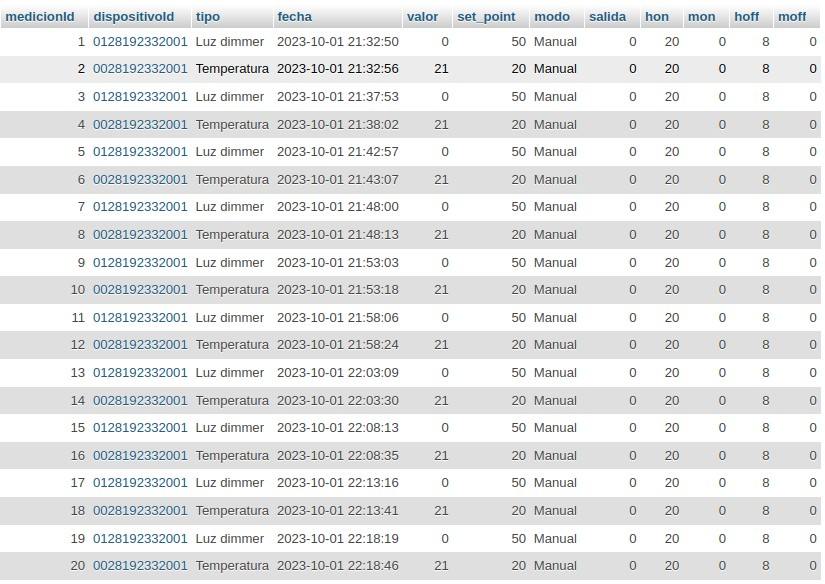
\includegraphics[scale=0.6]{Imagen 13 - Tabla mediciones.jpg}
\caption[Tabla mediciones]{Tabla de mediciones. \footnotemark}
\label{fig:13}
\end{figure}

\section{Desarrollo del frontend}

El frontend del presente trabajo fue desarrollado en el lenguaje TypeScript con Angular como \textit{framework} integrado con Ionic. El prototipo de aplicación está diseñado para acceder desde un navegador web tanto desde una computadora como un móvil, pero se optó por usar Ionic para un posterior desarrollo de una aplicación para sistemas operativos móviles. Es por esto que en esta instancia puede referirse a la aplicación web como una SPA y no como una PWA.

En la figura \ref{fig:14} se puede observar el fragmento de código correspondiente a la configuración de Ionic dentro del archivo \textit{docker-compose.yml}.

\begin{figure}[h]
\centering
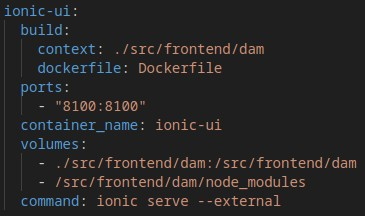
\includegraphics[scale=0.6]{Imagen 14 - Docker ionic.jpg}
\caption[Configuración Ionic]{Configuración de Docker de Ionic. \footnotemark}
\label{fig:14}
\end{figure}

La estructura de archivos de cada página esta diseñada de la misma forma como se muestra en la imagen \ref{fig:15}. Allí se pueden ver como ejemplo los archivos que componen la página \textit{home}.

\begin{figure}[h]
\centering
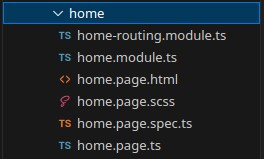
\includegraphics[scale=0.6]{Imagen 15 - Estructura.jpg}
\caption[Estructura página]{Estructura de archivos de página. \footnotemark}
\label{fig:15}
\end{figure}

Además se utilizaron interfaces para definir las estructuras de datos de los dispositivos, las mediciones y los usuarios, y servicios para el proceso de autenticación y de consultas HTTP al backend, que serán explicadas posteriormente.

El servicio de autenticación consta de el ingreso de un usuario y contraseña en la página de \textit{login} que se comparan con los que están almacenados en la base de datos. Si dichos valores ingresados corresponden con alguno de los existentes, se genera un \textit{token} desde el backend que se almacena en el dispositivo que está haciendo la consulta. Esto permite que se puedan acceder a las demás páginas de la aplicación.

En el código \ref{lst:Autenticación de rutas} puede verse el fragmento de la autenticación del archivo \textit{auth.guard.ts}

\definecolor{dkgreen}{rgb}{0,0.6,0}
\definecolor{gray}{rgb}{0.5,0.5,0.5}
\definecolor{mauve}{rgb}{0.58,0,0.82}

\lstset{frame=tb,
  language=Java,
  aboveskip=3mm,
  belowskip=3mm,
  captionpos=b,
  showstringspaces=false,
  columns=flexible,
  basicstyle={\small\ttfamily},
  numbers=left,
  numberstyle=\tiny\color{gray},
  keywordstyle=\color{blue},
  commentstyle=\color{dkgreen},
  stringstyle=\color{mauve},
  breaklines=true,
  breakatwhitespace=true,
  tabsize=3,
}

\begin{lstlisting}[caption={Autenticación de rutas}, label={lst:Autenticación de rutas}]
export class AuthGuard {
  constructor(private _loginService: LoginService, private _router: Router) {}
  canActivate(
    route: ActivatedRouteSnapshot,
    state: RouterStateSnapshot): Observable<boolean | UrlTree> | Promise<boolean | UrlTree> | boolean | UrlTree {
    if (!this._loginService.logIn) {
      this._router.navigate(['/login'])
      return false
    }
    return true;
  }
}
\end{lstlisting}

El \textit{route guard} es una característica del Angular Router que permite ejecutar algún tipo de lógica cuando se solicita una ruta, y basado en esa lógica, se permite o denega el acceso al usuario a esa ruta. Comúnmente es utilizado para verificar si un usuario está logueado o no en el sistema para verificar si tiene autorización para acceder a esa URL.

El \textit{route guard} se puede agregar implementando la interfaz \textit{CanActivate} disponible en \textit{@angular/router} y allí implementar el método \textit{canActivate()} que contendrá la lógica para denegar o permitir el acceso a la ruta.\citep{22}

\subsection{Rutas y páginas más importantes}

Las rutas disponibles en la aplicación se describen en la tabla \ref{tab:rutas}. A través de ellas se navega dentro de la aplicación y se accede a las distintas pantallas. Estas rutas se encuentran definidas en el archivo \textit{app-routing.module.ts} donde además se hace referencia al módulo de la aplicación que debe abrirse al acceder a cada una de las rutas listadas.

\begin{table}[h]
\centering
\caption[Rutas]{Rutas de la aplicación}
\begin{tabular}{l l}
\toprule
\textbf{Ruta} 			& \textbf{Descripción}\\
\midrule
/login					& Pantalla de inicio de sesión\\
/home					& Pantalla principal con funciones y listado de dispositivos\\
/usuario/:userId			& Pantalla de edición de datos de usuario\\
/ayuda					& Pantalla de manual de usuario\\
/dispositivos/:id		& Pantalla de visualización de estado del dispositivo\\
/medicion/:id			& Pantalla de visualización de las mediciones del\\
/grafico/:id				& Pantalla de visualización del gráfico de las mediciones\\
/config/:id				& Pantalla de configuración del dispositivo\\
/modificar/:id			& Pantalla de edición de datos de un dispositivo existente\\
/agregar					& Pantalla para agregar un dispositivo nuevo\\
\bottomrule
\hline
\end{tabular}
\label{tab:rutas}
\end{table}

En los casos en los que se encuentra el campo \textit{:id}, este valor se completa con el valor de identificador del elemento en cuestión. En el caso de los usuarios, cada uno de ellos tiene un identificador, lo mismo que para los dispositivos. Para las rutas \textit{medicion}, \textit{grafico}, \textit{config} y \textit{modificar} el \textit{:id} al que se hace referencia es el del dispositivo al que se quiere leer o modificar.

\subsubsection{Pantalla de \textit{login}}

En la figura \ref{fig:16} se muestra la página de inicio de sesión en la aplicación.

\begin{figure}[h]
\centering
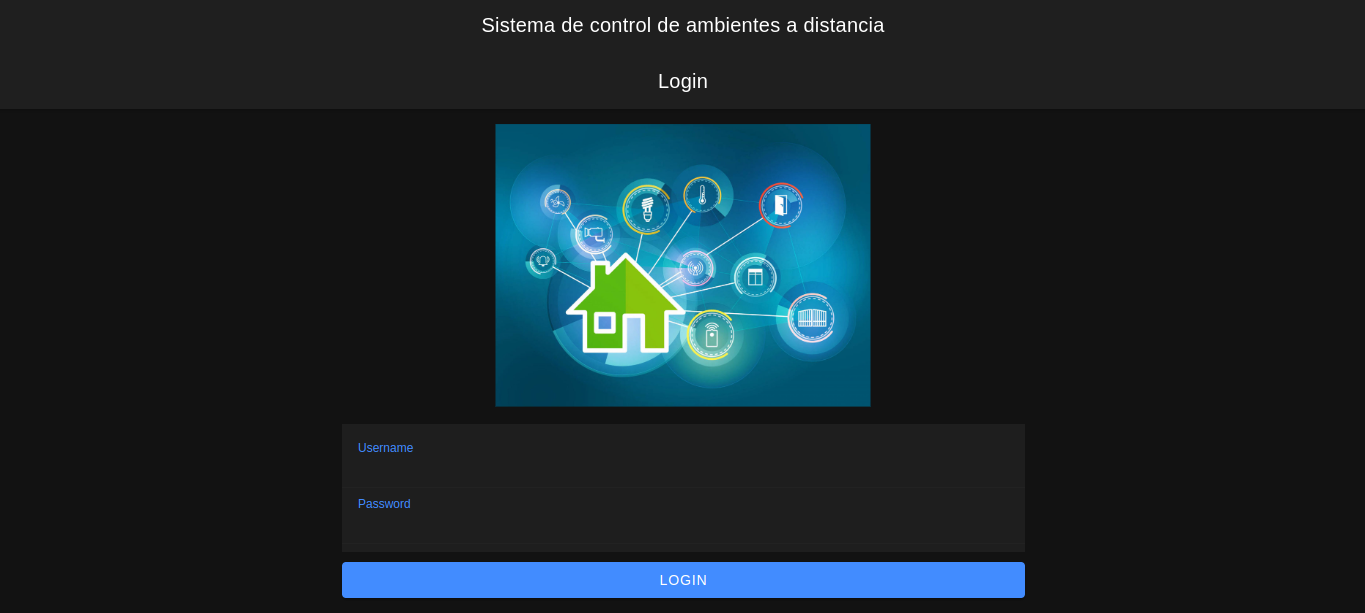
\includegraphics[scale=0.38]{Imagen 16 - Login.png}
\caption[Pantalla login]{Pantalla de \textit{login}. \footnotemark}
\label{fig:16}
\end{figure}

El sistema trae la posibilidad de configurar 3 usuarios distintos para que utilicen, visualicen y configuren la aplicación. Todos poseen el mismo rol y pueden configurar cualquier campo que corresponda a dicho usuario ingresando en la opción Usuario dentro de la pantalla principal.

\subsubsection{Pantalla principal \textit{home}}

En la figura \ref{fig:17} puede verse la pantalla principal de la aplicación. En la parte superior se encuentran los botones principales de la aplicación tales como el de configuración del usuario actual, cerrar sesión y la página de ayuda o manual de usuario. En la parte inferior se encuentra el listado de dispositivos implementado con \textit{ion-cards} los cuales permiten ver el estado de cada dispositivo, modificar los datos y alarma del dispositivo y eliminarlo de la lista. Hay que tener en cuenta que al borrar un dispositivo del sistema se borran también todas las mediciones y documentos asociados a él dentro de la base de datos.

\begin{figure}[h]
\centering
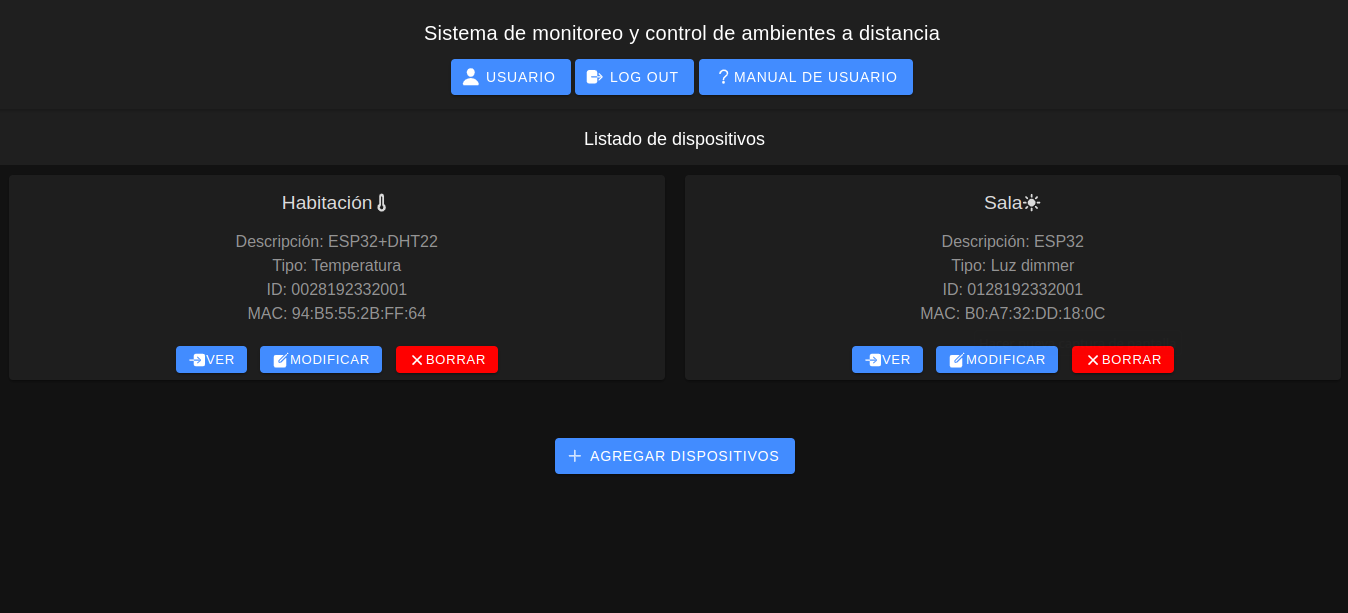
\includegraphics[scale=0.38]{Imagen 17 - Home.png}
\caption[Pantalla home]{Pantalla de \textit{home}. \footnotemark}
\label{fig:17}
\end{figure}

Por último en la parte inferior de la pantalla principal se encuentra el botón para agregar un dispositivo nuevo. Dicho botón dirige a la página de creación de un dispositivo nuevo.

\subsubsection{Pantalla de creación de dispositivo nuevo}

En la pantalla que se muestra en la figura \ref{fig:18} se deben cargar los datos de un dispositivo nuevo. Esto es importante ya que aquí se dan de alta los dispositivos nuevos que se incorporar al sistema.

\begin{figure}[h]
\centering
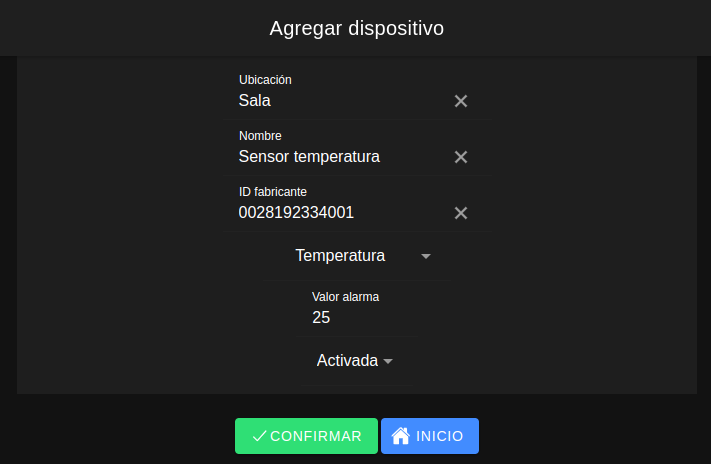
\includegraphics[scale=0.45]{Imagen 18 - Agregar.png}
\caption[Pantalla home]{Pantalla de creación de dispositivo nuevo. \footnotemark}
\label{fig:18}
\end{figure}

Aquí deben colocarse los datos de ubicación del nodo, el nombre con el que se desea identificarlo, el ID de fabricante, el tipo, y los valores de la alarma en caso de que se trate de un nodo de temperatura. El estado de la alarma puede configurarse pro primera vez en esta sección, pero puede modificarse cuando se desee. Se debe tener en cuenta que al momento existen 2 tipos de dispositivos: temperatura y luz dimmer. Solo se encuentra habilitada la alarma para los nodos del tipo de temperatura ya que no tiene sentido colocar una alarma a un nodo que no realiza mediciones ni controla parámetros críticos.

El ID del fabricante es un número de 13 dígitos compuesto de la siguiente forma: los 2 primeros identifican el tipo de dispositivo; los 4 que le siguen son obligatoriamente los números "2819", y se colocan como número de identificación del sistema y como seguridad; los 2 dígitos que le siguen son el año de fabricación del dispositivo; los 2 que le siguen son la semana de fabricación; y por último los 3 dígitos que restan son el número de fabricación en esa semana, es decir que comienza en el "000" y termina en "999". Este número resultante será entregado por el fabricante y será único para cada dispositivo.

Desde el frontend se verifica que se ingrese el código de seguridad dentro del ID del fabricante en el fragmento de código \ref{lst:Verificación de ID}:

\begin{lstlisting}[caption={Verificación de ID}, label={lst:Verificación de ID}]
verificarID(dispositivoId: string): boolean {
    const posicion = 2;
    return dispositivoId.charAt(posicion) === '2' &&
      dispositivoId.charAt(posicion + 1) === '8' &&
      dispositivoId.charAt(posicion + 2) === '1' &&
      dispositivoId.charAt(posicion + 3) === '9';
  }
\end{lstlisting}

Una vez que el dispositivo nuevo esté dado de alta, al encenderlo se va a conectar a la red y va a registrar automáticamente la dirección MAC dejándola guardada en la tabla de dispositivos.

\subsubsection{Pantalla de configuración de modo}

En esta sección se va a configurar el modo de trabajo y todos los parámetros asociados.

\begin{figure}[h]
\centering
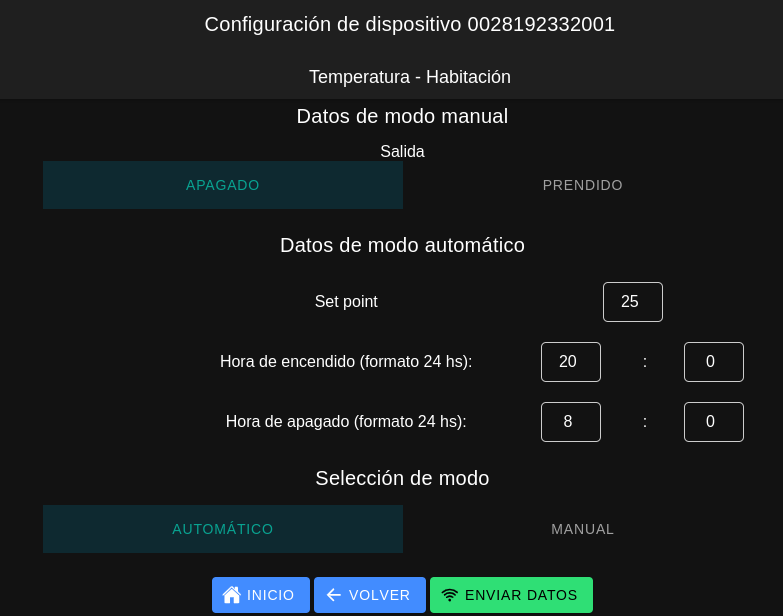
\includegraphics[scale=0.45]{Imagen 19 - Enviar datos.png}
\caption[Pantalla de configuración de modo]{Pantalla de configuración de modo. \footnotemark}
\label{fig:19}
\end{figure}

\section{Desarrollo del backend}



\section{Nodos, sensores y actuadores}

Los nodos están compuestos por el módulo central y los periféricos de entrada y salida. En el desarrollo del prototipo se utilizaron 2 versiones de módulo central, una que cuenta con un microcontrolador ESP32 para el nodo que controla temperatura y otra que cuenta con un ESP32 para el nodo que controla la iluminación dimerizable. En la tabla \ref{tab:esp32} pueden verse las características más importantes de ambos modelos de microcontroladores.

\begin{table}[h]
\centering
\caption[Módulos ESP32]{Especificaciones técnicas de los módulos ESP32.}
\begin{tabular}{l c c}
\toprule
\textbf{Característica} & \textbf{ESP32} & \textbf{ESP32C3}\\
\midrule
Núcleo			& Xtensa® dual-core 32-bit LX6 	& 32-bit single-core RISC-V \\
				& @240 MHz						& @160 MHz \\
Flash			& 0 MB, 2 MB o 4MB				& 0 MB o 4 MB \\
				& (dependiendo la versión)		& (dependiendo la versión) \\
Protocolo Wi-Fi	& 802.11 b/g/n, 2.4 GHz			& 802.11 b/g/n, 2.4 GHz \\
\bottomrule
\hline
\end{tabular}
\label{tab:esp32}
\end{table}

A continuación se listan periféricos utilizados como sensores y actuadores con sus principales características:
\begin{itemize}
	\item DHT22: sensor de temperatura y humedad relativa ambiente.
	\begin{itemize}
		\item Rango de temperatura: -40 a 80 grados Celsius.
		\item Resolución: 0,1 grado Celsius.
		\item Comunicación: serie, bus de 1 hilo, 40 bits por trama.
	\end{itemize}
	\item KY-040: encoder rotativo con interruptor cuya función es cambiar los parámetros desde el nodo. 20 pulsos por vuelta.
	\item SSD1306: display OLED 1,2 pulgadas.
	\begin{itemize}
		\item Resolución: 128x64 píxeles.
		\item Interfaz: I2C.
	\end{itemize}
	\item Control de potencia para 220 V: módulo con aislación y salida de triac para control de la calefacción. Se puede utilizar también para cualquier tipo de carga de 220 V 50 Hz.
	\begin{itemize}
		\item Tipo: encendido - apagado (on - off).
		\item Carga máxima: 8 A.
		\item Tipo de aislación: optoacoplador.
		\item Tensión máxima de aislación: 7500 V AC pico, 1 segundo de duración.
	\end{itemize}
	\item Control de intensidad de luz: módulo de control para iluminación LED de corriente continua implementado con modulación por ancho de pulso (PWM). También se puede utilizar como módulo de encendido y apagado para cualquier tipo de cargas de corriente continua.
	\begin{itemize}
		\item Tipo: PWM y encendido - apagado (on - off).
		\item Carga máxima: 800 mA CC.
		\item Tensión de alimentación: 5 a 24 V CC.
	\end{itemize}
\end{itemize}

En la imagen 2.4 puede observarse el diagrama en bloques del nodo de temperatura y control de calefacción. Los periféricos de entrada son el encoder y el sensor de temperatura y los de salida son el display que muestra la información y la salida de potencia.

\begin{figure}[h]
\centering
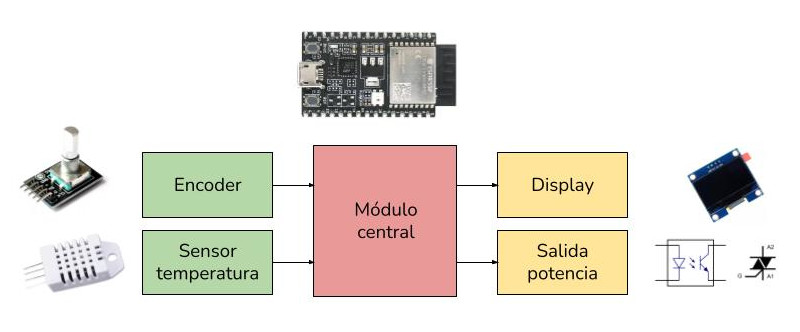
\includegraphics[scale=2]{Imagen 7 - Nodo temperatura.jpg}
\caption[Nodo de temperatura]{Diagrama en bloques del nodo de temperatura.}
\label{fig:4}
\end{figure}

En la figura 2.5 puede verse el diagrama en bloques del nodo de dimerización de la luminaria de corriente continua. En este caso, a diferencia del modelo descripto antes, posee un solo periférico de entrada y el de salida controla una salida de corriente continua de 5 a 24 V. En el caso del proyecto se utilizó una luminaria de 5 V y un consumo de 200 mA.

\begin{figure}[h]
\centering
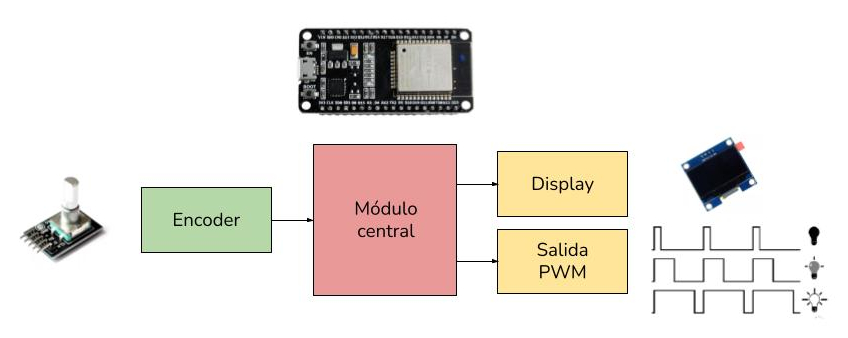
\includegraphics[scale=2]{Imagen 8 - Nodo dimmer.jpg}
\caption[Nodo dimer]{Diagrama en bloques del nodo de dimerización.}
\label{fig:4}
\end{figure}

\section{Comunicación del sistema}